


\section{FP4 Attention for Inference Acceleration}
This section presents our microscaling \texttt{FP4} attention through three key components: (1) the fundamental workflow for applying microscaling \texttt{FP4} quantization to attention in Section~\ref{sec:micro_scaling_fp4}, (2) the two-level quantization approach for the attention map in Section~\ref{sec:two_level_quant}, and (3) critical hardware implementation optimization in Section~\ref{sec:hardware_implement}.

\begin{figure}[ht]
    \centering
    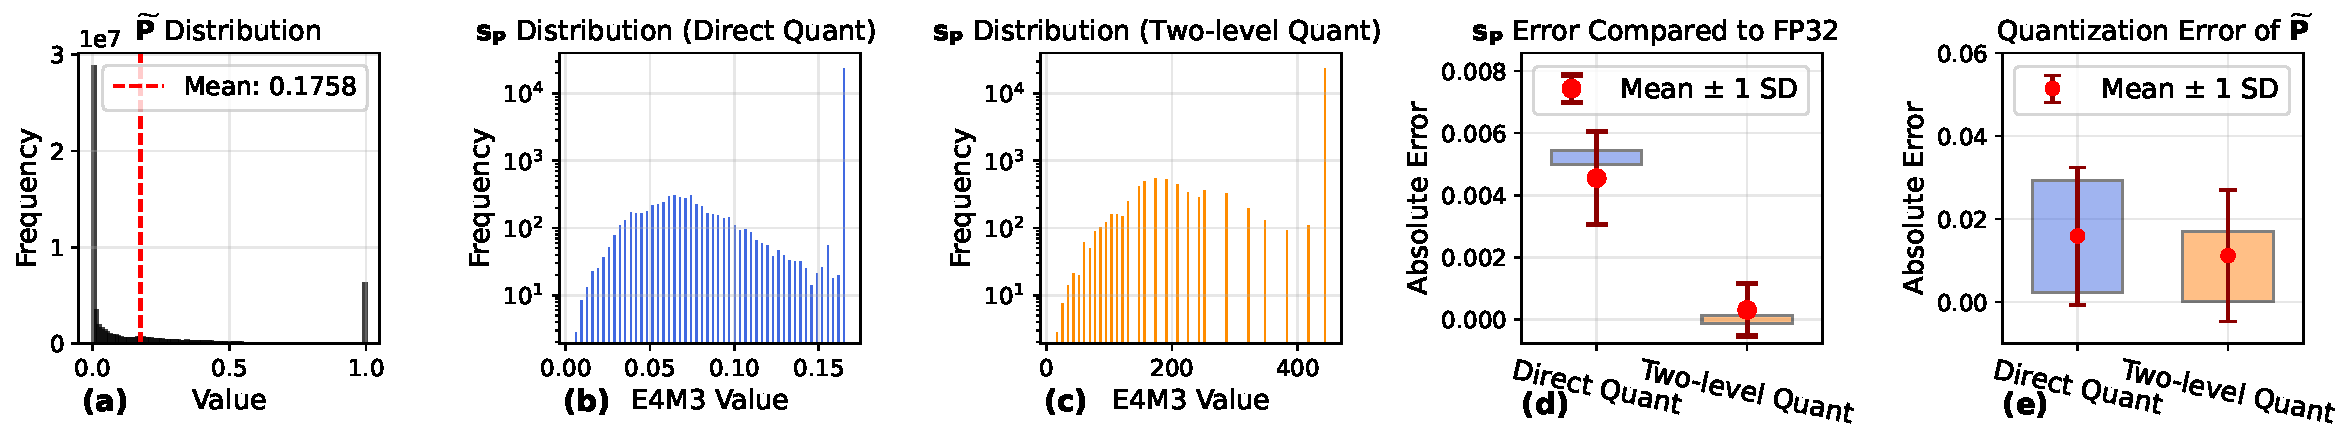
\includegraphics[width=1.01\columnwidth]{src/figs/quant_errors_of_p.pdf} 
    \vspace{-.5em}
    \caption{Analysis of the benefit of two-level quantization. (a) shows the distribution of $\widetilde \vP$. (b) and (c) show the distribution of $\mathbf{s_P}$ using direct quantization and two-level quantization. (d) and (e) show the error of $\mathbf{s_P}$ and $\widetilde \vP$ using direct quantization and two-level quantization.}
    \label{fig:quant_errors_of_p} 
\end{figure}



\subsection{Microscaling {FP4} Attention}  \label{sec:micro_scaling_fp4}
% We formulate the Microscaling \texttt{FP4} Attention as follows.

\textbf{FP4 microscaling quantization}. Given a matrix $X \in \mathbb{R}^{N \times d}$, we quantize it to $\hat X$ in \texttt{FP4} data type with a scale factor matrix $s_X$ in \texttt{FP8} data type. Specifically, $X$ is partitioned into $X_{ij} \in \mathbb{R}^{1 \times n}$ blocks, where each $1 \times n$ block corresponds to one scale factor $s_{ij}$. The \texttt{FP4} microscaling quantization ($[\hat X, s_X = \phi(X)]$) and dequantization ($X' = \phi^{-1}(\hat X, s_X)$) can be formulated as follows.
\begin{align}
    \textbf{Quantization $\phi$:}~&   s_{ij} = \max(|X|)/6, ~~~   \hat X_{ij} =   \lceil X_{ij} / s_{ij} \rfloor  \\
    \textbf{Dequantization $\phi^{-1}$:}~& ~ X_{ij}' = s_{ij} \times \hat X_{ij}
    \label{equ:microscaling} 
\end{align}

Where the $\lceil \cdot \rfloor$ means \texttt{FP4} rounding.


\textbf{FP4 microscaling quantization Matmul}. Consider a matrix multiplication $AB$, where $A$ and $B$ are in \texttt{FP16} precision. The speed of the Matmul is about 200 \texttt{TOPS} on \texttt{RTX5090}. In contrast, the speed of the \texttt{FP4} microscaling Matmul is about 1600 \texttt{TOPS}, which is an 8x speedup. The \texttt{FP4} microscaling Matmul instruction (\texttt{FP4MM}) takes four inputs, i.e., $\hat A, s_A, \hat B, s_B$, and the output $C$ equals to the Matmul result between $\phi^{-1}(\hat A, s_A)$ and $\phi^{-1}(\hat B, s_B)$:
\begin{align}
    C = \texttt{FP4MM}(\hat A, s_A, \hat B, s_B)
    \label{equ:FP4MM} 
\end{align}
\textbf{Attention computation.} We accelerate attention computation by applying \texttt{FP4} microscaling quantization to both matrix multiplications: $\vQ\vK^\top$ and $\vP\vV$. 
\begin{align}
    \hat \vQ, \mathbf{s_Q} = \phi(\vQ), ~~~
    \hat \vK, \mathbf{s_K} =& \phi(\vK^\top), ~~~
    \vS = \texttt{FP4MM}(\hat \vQ, \mathbf{s_Q}, \hat \vK, \mathbf{s_K})  \notag \\
    \widetilde \vP =& \texttt{OnlineSoftmax}(\vS)  \notag \\
    \hat \vP, \mathbf{s_P} = \phi(\widetilde \vP), ~~~
    \hat \vV, \mathbf{s_V} =& \phi(\vV), ~~~~~~
    \vO = \texttt{FP4MM}(\hat \vP, \mathbf{s_P}, \hat \vV, \mathbf{s_V}) 
\end{align}

It is important to note that our hardware implementation builds on FlashAttention, where the matrices $\vQ$, $\vK$, $\widetilde \vP$, and $\vV$ in our formulation correspond to FlashAttention’s tiled $Q$, $K$, $\widetilde{P}$, and $V$ blocks as described in Section~\ref{sec:preliminary}. Additionally, to enhance the attention accuracy, we adopt the smoothing $Q$ and $K$ in SageAttention2~\citep{zhang2024sageattention2}. The complete algorithm is presented in Algorithm~\ref{alg:sage3_fwd}.


\textbf{Data type determination.} 
There are two choices for the \texttt{FP4} data type~\citep{rouhani2023microscaling}. The first one is the \texttt{NVFP4}, which is in \texttt{E2M1} data type and its quantization block size is $1 \times 16$ and its scale factor is in \texttt{E4M3} data type. The second one is the \texttt{MXFP4}, which is also in \texttt{E2M1} data type. However, its quantization block size is $1 \times 32$ and its scale factor is in \texttt{E8M0} data type. We choose \texttt{NVFP4} 
because the accuracy of \texttt{NVFP4} is much higher than that of \texttt{MXFP4} in attention quantization. \underline{Empirical results:} Table~\ref{tab:acc_ablation}(\subref{table:a}) shows the accuracy of \texttt{MXFP4} and \texttt{NVFP4} using real \textbf{Q, K, V} across all layers of \texttt{CogVideoX}. Results indicate that the accuracy of \texttt{NVFP4} outperforms that of \texttt{MXFP4}.

% \begin{table}[h]
% \caption{\textbf{Average accuracy} and \textbf{Worst accuracy} accross all layers of \texttt{CogVideoX} using different data types.}
% \centering
% \begin{minipage}{0.48\linewidth}
% \centering
% \textbf{Average}
% \begin{tabular}{lccc}
% \toprule
%         & \textbf{CosSim} & \textbf{L1} & \textbf{RMSE} \\
% \midrule
% \texttt{MXFP4}   & 99.21\% & 0.2350   & 0.4649 \\
% \texttt{NVFP4}   & 99.87\% & 0.0774 & 0.2013 \\
% \bottomrule
% \end{tabular}
% \end{minipage}
% \hfill
% \begin{minipage}{0.48\linewidth}
% \centering
% \textbf{Worst}
% \begin{tabular}{lccc}
% \toprule
%         & \textbf{CosSim} & \textbf{L1} & \textbf{RMSE} \\
% \midrule
% \texttt{MXFP4}   & 98.37\% & 0.2941 & 0.9944 \\
% \texttt{NVFP4}   & 99.52\% & 0.0774 & 0.2013 \\
% \bottomrule
% \end{tabular}
% \end{minipage}
% \label{table:mxfp4}
% \end{table}



\begin{algorithm}[ht]
    \small
    \caption{Implementation of the microscaling \texttt{FP4} attention.}
    \label{alg:sage3_fwd} 
    % \setlength{\textfloatsep}{-10pt}
    \begin{algorithmic}[1]
    \STATE {\bfseries Input:} {Matrices $Q(\texttt{FP16}), K(\texttt{FP16}), V(\texttt{FP16}) \in \mathbb{R}^{N \times d}$, block size $B_q, B_{kv}$.}
    

    \STATE \textbf{Preprocessing:} \jt{$K=K-\mathrm{mean}(K)$} \annotate{// Smoothing K of SageAttention.}
    
    \STATE Divide $Q$ to $T_m = {N}/{B_q}$ blocks $\{\vQ_i\}$; divide $K$, and $V$ to $T_n = {N}/{B_{kv}}$ blocks $\{\vK_i\}$, $\{\vV_i\}$ ;  

    \FOR {$i=1$ {\bfseries to} $T_m$}

      \STATE $\jt{\bar q_i=\mean(\vQ_i),~~ (\mathbf{s_Q}, \hat \vQ_i)} = \jt{\phi(\vQ_i - \bar q_i)}$  ; \annotate{// Smoothing Q of SageAttention2.} 

        \FOR {$j$ in [1, $T_n$]} 
            \STATE $\jt{(\mathbf{s_K}, \hat \vK_j)} = \jt{\phi}(\vK_j^\top)$ , ~~ $\jt{(\mathbf{s_V}, \hat \vV_j)} = \jt{\phi}(\vV_j)$ ; 

            \STATE \jt{$\vS_{ij} = \texttt{FP4MM} (\hat \vQ_i, \mathbf{s_Q}, \hat \vK_j, \mathbf{s_K}) + \texttt{GEMV}(\bar q_i, \vK_j^\top)$} ;  \annotate{// Smoothing Q.}

            \STATE $m_{ij} = \mathrm{max}(m_{i,j-1}, \mathrm{rowmax}(\vS_{ij}))$, $~\widetilde \vP_{ij} = \mathrm{exp}(\vS_{ij} - m_{ij})$, $~l_{ij} = e^{m_{i,j-1}-m_{ij}} l_{i,j-1} + \mathrm{rowsum}(\widetilde \vP_{ij})$ ;

            \STATE \jt{$\mathbf{s_{P_1}} = \rowmax(\widetilde \vP_{ij}) / (448 \times 6)$, ~ $\widetilde \vP_{ij} = \widetilde \vP_{ij} / \mathbf{s_{P_1}}$, ~ $\mathbf{s_{P_2}}, \hat \vP_{ij} = \phi (\widetilde \vP_{ij})$}; \annotate{// two-level quantization}

            \STATE $\vO_{ij} = \mathrm{diag}(e^{m_{i,j-1}-m_{ij}}) \vO_{i,j-1} + \jt{\texttt{FP4MM}(\hat \vP_{ij}, \mathbf{s_{P_2}}, \hat \vV_j, \mathbf{s_V}) \times \mathbf{s_{P_1}}}$
        
        \ENDFOR
        \STATE $\vO_i = \mathrm{diag}(l_{i,T_n}) ^{-1} \vO_{i,T_n}$ ; %~~~ Write $\vO_i$ ;  
    \ENDFOR
    
    \STATE \textbf{return} $O = \{\vO_i\}$
    \end{algorithmic}
    \vspace{-.2em}
\end{algorithm}






\subsection{Two-level Scaling for $\widetilde \vP$}  \label{sec:two_level_quant}
Applying microscaling \texttt{FP4} quantization for $\widetilde \vP$ presents a challenge to attention accuracy. For example, Fig.~\ref{fig:scale_ablation}(~\subref{fig:c}) shows direct quantization severely degrades output quality, producing results substantially different from full-precision outputs. Our analysis reveals that the issue occurs because microscaling \texttt{NVFP4} quantization requires the scale factor to be represented in \texttt{E4M3} \texttt{FP8} format~\citep{micikevicius2022fp8}, rather than the \texttt{FP32} data type typically used for scale factors. This causes accuracy loss when the scale factor is directly converted to \texttt{E4M3} format. 
To better understand this accuracy loss, we analyze the data distribution of $\widetilde \vP$ and its scale factors in Fig.~\ref{fig:quant_errors_of_p}. 
Since $\widetilde \vP$ is computed using online softmax~\citep{milakov2018online}, the values in each microscaling block $\widetilde \vP_{ij}$ fall $\mathsf{[0, 1]}$. Consequently, the scale factor (scale factor = $\max(\widetilde \vP_{ij})/6$) ranges between 0 and 0.167. This narrow range leads to inefficient usage of \texttt{E4M3}'s representable range, increasing accuracy loss. To reduce accuracy loss by fully utilizing \texttt{E4M3}'s range, we propose a two-level quantization method for the $\widetilde \vP$ matrix. Specifically, we first quantize each row of $\widetilde \vP$ to $\mathsf{[0, 448 \times 6]}$. Then we apply the standard \texttt{FP4} quantization $\phi$ for the quantized $\widetilde \vP$. The two-level quantization can be formulated as follows:
\begin{align}
    \mathbf{s_{P_1}} = \rowmax(\widetilde \vP) / (448 \times 6), ~~~
    \widetilde \vP_2 &= \widetilde \vP / \mathbf{s_{P_1}}, ~~~
    \mathbf{s_{P_2}}, \hat \vP_2 = \phi (\widetilde \vP_2) \notag\\
    (\widetilde \vP \approx \hat \vP_2 \times \mathbf{s_{P_2}} \times \mathbf{s_{P_1}}), ~~~~
    \vO &= \texttt{FP4MM}(\hat \vP_2, \mathbf{s_{P_2}}, \hat \vV, \mathbf{s_V}) \times \mathbf{s_{P_1}}
\end{align}
Where $\widetilde \vP$, $\widetilde \vP_2$, and $\mathbf{s_{P_1}}$ are in \texttt{FP32} data type. $\mathbf{s_{P_2}}$ and $\mathbf{s_V}$ are in  \texttt{FP8}  data type. $\hat \vP_2$ and $\hat \vV$ are in \texttt{FP4} data type.


\underline{Empirical results:} As shown in Fig.~\ref{fig:quant_errors_of_p}, our two-level quantization maximizes the \texttt{E4M3} range utilization for $\mathbf{s_P}$, thereby reducing both the numerical representation error of $\mathbf{s_P}$ and the quantization error of $\widetilde{\vP}$. A more formal theoretical analysis is provided in Appendix~\ref{sec:appendix_others}. 
Table~\ref{tab:acc_ablation}(\subref{table:b}) shows the accuracy of two-level quantization against naive direct quantization, using real Q, K, V from layers of CogVideoX. Results indicate that two-level quantization boosts the accuracy.



% \begin{table}[h]
% \begin{minipage}{0.48\linewidth}
% \centering
% \caption{\textbf{Average accuracy} across all layers of \texttt{CogVideoX} using different data types.}
% \label{table:average_accuracy_dtype}
% \sisetup{
%     round-mode = places, 
%     round-precision = 3 
% }
% \begin{tabular}{
%     cc
%     S[table-format=2.2]
%     S[table-format=1.4]
%     S[table-format=1.4]
%     cc
% }
% \toprule
% \textbf{Type} & \textbf{CosSim} & \textbf{L1} & \textbf{RMSE} \\
% \midrule
% \texttt{MXFP4} & 99.21\% & 0.2350 & 0.4649 \\
% \texttt{NVFP4} & 99.87\% & 0.0774 & 0.2013 \\
% \bottomrule
% \end{tabular}
% \end{minipage}
% \hfill
% \begin{minipage}{0.48\linewidth}
% \centering
% \caption{\textbf{Worst accuracy} across all layers of \texttt{CogVideoX} using different data types.}
% \label{table:worst_accuracy_dtype}
% \sisetup{
%     round-mode = places, 
%     round-precision = 3 
% }
% \begin{tabular}{
%     cc
%     S[table-format=2.2]
%     S[table-format=1.4]
%     S[table-format=1.4]
%     cc
% }
% \toprule
% \textbf{Type} & \textbf{CosSim} & \textbf{L1} & \textbf{RMSE} \\
% \midrule
% \texttt{MXFP4} & 98.37\% & 0.2941 & 0.9944 \\
% \texttt{NVFP4} & 99.52\% & 0.0774 & 0.2013 \\
% \bottomrule
% \end{tabular}
% \end{minipage}
% \end{table}





% \begin{table}[h]
% \begin{minipage}{0.48\linewidth}

% \centering
% \caption{\textbf{Average accuracy} across all layers of \texttt{CogVideoX} using different scale strategies.}
% \label{table:average_accuracy_scale}
% \sisetup{
%     round-mode = places, 
%     round-precision = 3 
% }
% \begin{tabular}{
%     cc
%     S[table-format=2.2]
%     S[table-format=1.3]
%     S[table-format=1.3]
%     cc
% }
% \toprule
%  \textbf{Method}  & \textbf{CosSim} & \textbf{L1} & \textbf{RMSE} \\
% \midrule
% Direct Quantize         & 99.14\% & 0.0902 & 0.2492 \\
% Two-level Scale  & 99.87\% & 0.0774 & 0.2013 \\
% \bottomrule
% \end{tabular}
% \end{minipage}
% \hfill
% \begin{minipage}{0.48\linewidth}
% \centering
% \caption{\textbf{Worst accuracy} across all layers of \texttt{CogVideoX} using different scale strategies.}
% \label{table:worst_accuracy_scale}
% \sisetup{
%     round-mode = places, 
%     round-precision = 3 
% }
% \begin{tabular}{
%     cc
%     S[table-format=2.2]
%     S[table-format=1.3]
%     S[table-format=1.3]
%     cc
% }
% \toprule
%  \textbf{Method}       & \textbf{CosSim} & \textbf{L1} & \textbf{RMSE} \\
% \midrule
% Direct Quantize         & 93.32\% & 0.1925 & 1.1030 \\
% Two-level Scale  & 99.52\% & 0.0774 & 0.2013 \\
% \bottomrule
% \end{tabular}
% \end{minipage}
% \end{table}






% \jt{Need a visualized map or data distritbution related to the range of the scale factor.}



\subsection{Implementation and Optimization on Hardware}  \label{sec:hardware_implement}

\textbf{Permutation for K.}
Unlike \texttt{FP16}, the \texttt{FP32} accumulator's memory layout in \texttt{FP4} MatMul~\citep{nvidia2024ptx} differs from its operand A's register layout (shown in Fig. \ref{fig:ori_fp32_layout} and \ref{fig:input_layout}). Performing thread shuffles to match operand A's layout would degrade kernel performance.
Our solution transforms the accumulator layout (Fig. \ref{fig:new_fp32_layout}) by permuting the P tile's columns. To maintain correct MatMul, we correspondingly rearrange K's columns, which can be fused with the quantization kernel.


\textbf{Reuse shuffle.} 
The in-kernel micro-scaling quantization of $\widetilde \vP$ requires finding the max value of 16 consecutive row elements. However, as shown in Fig.~\ref{fig:new_fp32_layout}, these 16 elements are distributed across four threads, necessitating intra-thread max reduction followed by inter-thread shuffling, significantly slowing down the kernel.
We optimize this by fusing quantization with online softmax, which also computes row-wise maxima. First, we compute the max over 16 elements in $S$ and reuse it in the subsequent softmax max-reduction. This fusion reduces redundant shuffles and max operations by ~50\%, yielding about 10\% whole kernel speedup.
% The in-kernel micro-scaling quantization of $\widetilde \vP$ requires finding the absolute maximum of 16 consecutive row elements. However, as shown in Fig.~\ref{fig:new_fp32_layout}, these 16 elements are distributed across four threads, necessitating intra-thread absolute max reduction followed by inter-thread shuffling, significantly slowing down the kernel.
% We optimize this by fusing quantization with online softmax, which also computes row-wise maxima and maps all elements in $S$ to be positive. First, we compute the max over 16 elements in $S$. Note that this max need to be exponentiated to be the true value for micro-scaling quantization. Then we resue this maxia for continual online softmax. This fusion reduces redundant shuffles and max operations by ~50\%, with an neligble overhead of one extra exp operation, yielding about 10\% whole kernel speedup.



\textbf{Producer warp epilogue.} 
In conventional warp-specialized kernels, consumer warps typically handle both MatMul and store operations while producers merely load inputs, with ping-pong scheduling between consumers enabling stage overlap~\citep{nvidia2025efficientgemm}. However, register constraints make this approach infeasible for our \texttt{FP4} attention kernel. Instead, we implement ping-pong scheduling between producer warps: while one producer loads inputs for the next MatMul operation, another concurrently stores outputs to global memory, with consumer warps solely responsible for transferring MatMul results from registers to shared memory. This novel design overlaps MatMul and global memory stores within register constraints, boosting throughput.







